\csname @openrightfalse\endcsname
\chapter{Piecewise linear geometry}


A \index{polyhedral space}\emph{polyhedral space} is a complete length-metric space that admits a locally finite triangulation 
such that each simplex is isometric to a simplex in a Euclidean space.
By a {}\emph{triangulation} of a polyhedral space we always mean a triangulation of that type. 

A point in a polyhedral space is called \index{regular point}\emph{regular} if it has a neighborhood isometric to an open set in a Euclidean space;
otherwise it is called {}\emph{singular}.

If we replace the Euclidean spaces by the unit spheres or the hyperbolic spaces,
we arrive at the definition of {}\emph{spherical} and {}\emph{hyperbolic polyhedral spaces} respectively.

The term \index{piecewise}\emph{piecewise} typically means that there is a triangulation with some property on each triangle.
For example,  if $P$ and $Q$ are polyhedral spaces, then
\begin{itemize}
\item a map $f\:P\to Q$ is called {}\emph{piecewise distance preserving} if there is a triangulation $\mathcal{T}$ of $P$ such that for any simplex $\Delta\in \mathcal{T}$ the restriction $f|_\Delta$ is distance preserving;
\item a map $h\:P\z\to Q$  is called {}\emph{piecewise linear} if both spaces $P$ and $Q$ admit triangulations such that each simplex of $P$ is mapped to a simplex of $Q$ by an affine map.
In particular, a {}\emph{piecewise linear homeomorphism} is a piecewise linear map which is a homeomorphism.\label{piecewise linear map}
\end{itemize}





%%%%%%%%%%%%%%%%%%%%%%%%%%%%%%%%%%%%%%%%%
\subsection*{Spherical arm lemma}\label{Spherical arm lemma}

Recall that a polygon without self intersections is called \index{simple polygon}\emph{simple}.

\begin{pr}
Let $A=[a_1\dots a_n]$ and $B=[b_1\dots b_n]$ be two simple spherical polygons 
with equal corresponding sides.
Assume that $A$ lies in a hemisphere and $\measuredangle a_i\ge\measuredangle b_i$ for each $i$.
Show that $A$ is congruent to $B$.
\end{pr}

%%%%%%%%%%%%%%%%%%%%%%%%%%%%%%%%%%%%%%%%%%%%%%%%%%
\parit{Semisolution.}
Let us cut out the polygon $A$ from the sphere and glue the polygon $B$ in its place.
Denote by $\Sigma$ the obtained spherical polyhedral space.
Note that 
\begin{itemize}
\item $\Sigma$ is homeomorphic to $\mathbb S^2$.
\item $\Sigma$ has curvature $\ge 1$ in the sense of Alexandrov; that is, the total angle around each singular point is less than $2\cdot \pi$.
\item All the singular points of $\Sigma$ 
lie outside of an isometric copy of a hemisphere $\mathbb{S}^2_+\subset \Sigma$.
\end{itemize}

Denote by $n$ the number of singular points in $\Sigma$.
It is sufficient to show that $n=0$.

Assume the contrary; that is, $n\ge 1$.
We can assume that $n$ takes the minimal possible value.

Clearly $n>1$;
that is, $\Sigma$ cannot have a single singular point.
Therefore we can choose two singular points $p,q\in \Sigma$.
Cut $\Sigma$ along a geodesic $[pq]$.
The obtained hole can be patched so that we obtain a new polyhedral space $\Sigma'$ of the same type but with $n-1$ singular points.
Since $n$ is minimal, we arrive at a contradiction.

Namely, if the total angles around $p$ and $q$ are $2\cdot \pi-\alpha$ and $2\cdot \pi-\beta$ respectively,
consider the spherical triangle $\triangle$ with the base $|p\z-q|_\Sigma$ and the adjacent angles $\tfrac\alpha2$, $\tfrac\beta2$. 
The needed patch is obtained by doubling $\triangle$ along its lateral sides.
\qeds

\parit{Alternative end of proof.}
By the Alexandrov embedding theorem, $\Sigma$ is isometric to the surface of a convex polyhedron $P$ in the unit sphere $\mathbb S^3$. 
The center of the hemisphere has to lie in a facet of $P$, say $F$.
It remains to note that $F$ contains the equator and therefore $P$ has to be a hemisphere in $\mathbb S^3$ or an intersection of two hemispheres.
In both cases its surface is isometric to $\mathbb S^2$.
\qeds

The problem is due to Victor Zalgaller \cite{zalgaller-shperical-polygon};
the result of Victor Toponogov in \cite{toponogov} gives a smooth analog of this statement.
The patch construction above was introduced by 
Aleksandr Alexandrov
in his proof of convex embeddability of polyhedra
\cite[see VI, \S7 in][]{alexandrov1948}.
The alternative end of the proof is taken from \cite{panov-petrunin}.



%%%%%%%%%%%%%%%%%%%%%%%%%%%%%%%%%%%%%%%%%
\subsection*{Triangulation of 3-sphere}\label{4-poly}

\begin{pr}
Construct a triangulation of $\mathbb{S}^3$ 
with $100$ vertices
such that any two vertices are connected by an edge.
\end{pr}

%%%%%%%%%%%%%%%%%%%%%%%%%%%%%%%%%%%%%%%%%
\subsection*{Folding problem}\label{Folding problem}

\begin{pr}
Let $P$ be a compact $2$-dimensional 
polyhedral space. 
Construct a 
piecewise distance preserving map
$f\:P\to \RR^2$.
\end{pr}

%%%%%%%%%%%%%%%%%%%%%%%%%%%%%%%%%%%%%%%%%
\subsection*{Piecewise distance preserving extension}\label{iso-kirzhbraun}

\begin{pr}
Prove that any 1-Lipschitz map from a finite subset $F\subset \RR^2$
to 
$\RR^2$ can be extended to a 
piecewise distance preserving map
$\RR^2\to\RR^2$.
\end{pr}

%%%%%%%%%%%%%%%%%%%%%%%%%%%%%%%%%%%%%%%%%
\subsection*{Closed polyhedral surface}\label{Closed polyhedral surface}

\begin{pr}
Construct a closed polyhedral surface $\Sigma$ in $\RR^3$ with nonpositive curvature;
that is, the total angle around each vertex of $\Sigma$ is at least~$2\cdot\pi$.
\end{pr}

%%%%%%%%%%%%%%%%%%%%%%%%%%%%%%%%%%%%%%%%%
\subsection*{Minimal polyhedral disk}\label{Minimal polyhedral disk}

By a polyhedral disk in $\RR^3$
we mean a triangulation of a plane polygon $P$ with a map $P\to\RR^3$ that is affine on each triangle.
The area of the polyhedral disk is defined as the sum of areas of the images of the triangles in the triangulation.

\begin{pr}
Consider the  class of polyhedral disks glued from $n$ triangles in $\RR^3$ 
with a fixed broken line as the boundary.
Let $\Sigma_n$ be a disk of minimal area in this class.
Show that $\Sigma_n$ is a \index{saddle surface}\emph{saddle surface};
that is, a plane cannot cut all the edges coming from one of the interior vertices of~$\Sigma_n$.
\end{pr}

%%%%%%%%%%%%%%%%%%%%%%%%%%%%%%%%%%%%%%%%%
\subsection*{Coherent triangulation\easy}\label{Coherent triangulation} 

A triangulation of a convex polygon is called coherent if there is a convex function that is linear on each triangle and changes its gradient on every edge of the triangulation.

\begin{pr}
Find a non-coherent triangulation of a triangle.
\end{pr}



%%%%%%%%%%%%%%%%%%%%%%%%%%%%%%%%%%%%%%%%%
\subsection*{Sphere with one edge\hard}\label{panov-S^3} 

Given  a polyhedral space $P$,
denote by $P_s$ the set of its 
singular points.

\begin{pr}
Construct spherical polyhedral space $P$ that is homeomorphic to $\mathbb{S}^3$ and such that $P_s$ is formed by a knotted circle.
\end{pr}

In addition, the total length of $P_s$ can be made arbitrarily large and the angle around $P_s$ can be made strictly less than $2\cdot\pi$.

%%%%%%%%%%%%%%%%%%%%%%%%%%%%%%%%%%%%%%%%%
\subsection*{Triangulation of a torus}\label{Triangulation of a torus}

\begin{pr}
Show that a torus does not admit a triangulation 
such that one vertex has 5 edges,
one has 7 edges and 
all other vertices have 
6 edges. 
\end{pr}


%%%%%%%%%%%%%%%%%%%%%%%%%%%%%%%%%%%%%%%%%
\subsection*{No simple geodesics\easy}\label{No simple geodesics}

\begin{pr}
Construct a convex polyhedron $P$ whose surface 
does not have a closed simple geodesic.
\end{pr}

\section*{Semisolutions}
%%%%%%%%%%%%%%%%%%%%%%%%%%%%%%%%%%%%%%%%%%%%%%%%%%


%%%%%%%%%%%%%%%%%%%%%%%%%%%%%%%%%%%%%%%%%%%%%%%%%%
\parbf{Triangulation of 3-sphere.}
Choose 100 distinct points $p_1\z\dots,p_{100}$
on the {}\emph{moment curve} 
\[\gamma\:t\mapsto (t,t^2,t^3,t^4)\] 
in $\RR^4$.
Denote by $P$ the convex hull of $\{p_1,\z\dots,p_{100}\}$.

The surface of $P$ is homeomorphic to $\mathbb{S}^2$.
Therefore it is sufficient to show that any two vertices of $P$ are connected by an edge.
The latter follows from the following claim.

\begin{cl}{$({*})$}
Given two points $p$ and $q$ on $\gamma$, there is a hyperplane $H$ in $\RR^4$ that intersects $\gamma$ only at $p$ and $q$ and leaves $\gamma$ on one side.
\end{cl}

To prove the claim, assume that $p=\gamma(t_1)$ and $q=\gamma(t_2)$. 
Consider the polynomial
\[f(t)=a+b\cdot t+c\cdot t^2+d\cdot t^3+t^4=(t-t_1)^2\cdot(t-t_2)^2.\]
Clearly $f(t)\ge 0$ and the equality holds only at $t_1$ and $t_2$.
It follows that the affine function $\ell\:\RR^4\to\RR$ defined by 
\[\ell\:(w,x,y,z)\mapsto a+b\cdot w+c\cdot x+d\cdot y+z\]
is nonnegative at the points of $\gamma$ and vanish only at $p$ and $q$.
Therefore the zero set of $\ell$ is the required hyperplane $H$ in $({*})$. 
\qeds

The polyhedron $P$ above is an example of the so-called \index{cyclic polytope}\emph{cyclic polytopes}.

%%%%%%%%%%%%%%%%%%%%%%%%%%%%%%%%%%%%%%%%%%%%%%%%%%
\parbf{Folding problem.}
Given a triangulation of $P$,
consider the Voronoi domain $V_v$ for each vertex $v$;
that is, $V_v$ is the set of all points in $P$ closer to $v$ than to any other vertex.
Note that the triangulation can be subdivided if necessary
so that the Voronoi domain of each vertex is isometric to a convex subset in the cone with the vertex at its tip.

The boundaries of all the Voronoi domains form a graph with straight edges.
Let us triangulate $P$ so that each triangle has one of those edges as the base 
and the opposite vertex is the center of an adjacent Voronoi domain; 
such a vertex will be called the {}\emph{main} vertex of the triangle.

\begin{wrapfigure}[7]{o}{47 mm}
\vskip-0mm
\centering
\includegraphics{mppics/pic-802}
\end{wrapfigure}

Choose a solid triangle $\triangle=[vab]$ in the constructed triangulation; 
let $v$ be its main vertex.
Given a point 
$x\in  \triangle$, set 
\begin{align*}
\rho(x)&=|x-v|
\intertext{and}
\theta(x)&=\min \{\measuredangle \hinge vax,\measuredangle\hinge vbx\}.
\end{align*}
Let us map $x$ to the point with polar coordinates $(\rho(x),\theta(x))$ in the plane.

Note that for each triangle $\triangle$, 
the constructed map $\triangle\to\RR^2$ is piecewise distance preserving.
It remains to check that these maps agree on the common sides of the triangles.
\qeds

This construction was given by Victor Zalgaller \cite{zalgaller-polyhedra}.
Svetlana Krat generalized the statement to higher dimensions \cite{krat}.



%%%%%%%%%%%%%%%%%%%%%%%%%%%%%%%%%%%%%%%%%%%%%%%%%%
\parbf{Piecewise distance preserving extension.}
Let $a_1,\dots,a_n$
and $b_1,\z\dots,b_n$
be two collections of points in $\RR^2$
such that 
\[|a_i-a_j|\ge |b_i-b_j|\] 
for all pairs $i$, $j$.
We need to construct a piecewise distance preserving map $f\:\RR^2\to\RR^2$
such that $f(a_i)=b_i$ for each $i$.

Assume that the problem is already solved for $n<m$;
let us do the case $n=m$.
By assumption, 
there is a piecewise linear length-preserving map $f\:\RR^2\to\RR^2$
such that $f(a_i)=b_i$ for each $i>1$.

Consider the set 
\[\Omega=\set{x\in\RR^2}{|f(x)-b_1|>|x-a_1|}.\]
Since $|a_i-a_1|\ge|b_i-b_1|$, we get $a_i\notin \Omega$ for $i>1$.

Note that we can assume that the map $f$ and therefore the set $\Omega$ are bounded.
Indeed, let $\square$ be a square containing all the points $b_i$.
There is a piecewise isometric map $h\:\RR^2\to\square$ obtained by folding plane along the lines of the grid defined by $\square$.
Then the composition $h\circ f$ is bounded and it satisfies all the properties of $f$ described above.

If $\Omega=\emptyset$,
then $f(a_1)=b_1$; 
that is, $f$ is a solution.
It remains to consider the case $\Omega\ne\emptyset$. 

Note that $\Omega$ is star-shaped with respect to $a_1$.
Indeed, if $x\in \Omega$, then $|a_1-x|<|b_1-f(x)|$.
If $y\in [a_1x]$ then 
$|a_1-y|+|y-x|=|a_1-x|$ and since $f$ is length-preserving we get $|f(x)-f(y)|\le |x-y|$.
By the triangle inequality, 
$|a_1-y|<|b_1-f(y)|$; that is, $y\in\Omega$. 

\begin{wrapfigure}{o}{47 mm}
\vskip-0mm
\centering
\includegraphics{mppics/pic-804}
\end{wrapfigure}

The boundary $\partial\Omega$ can be subdivided into a finite collection of line segments $\{E_i\}$
so that $f$ maps rigidly each $E_i$.
Note that 
\[|f(x)\z-b_1|=|x-a_1|\]
for any $x\in E_i$.
Denote by $T_i$ the triangle with the base $E_i$ and the vertex $a_1$.
From the above there is a rigid motion $m_i$ of $T_i$ such that $m_i(x)\z=f(x)$ for any $x\in E_i$ and $m_i(a_1)=b_1$.
Let us redefine the map $f$ in $\Omega$ by sending $x$ to $m_i(x)$ for any $x\in T_i$.

The maps $m_i$ agree on the common sides of triangles $T_i$.
Therefore we have produced a new piecewise isometric map $f'\:\RR^2\to \RR^2$ satisfying all the requirements.
\qeds

The same proof works in all dimensions.

The statement was proved by Ulrich Brehm 
and rediscovered by Arseniy Akopyan and Alexey Tarasov [see \ncite{brehm}, \ncite{akopyan-tarasov}, and Section 2 in \ncite{petrunin-yashinsky}].

%%%%%%%%%%%%%%%%%%%%%%%%%%%%%%%%%%%%%%%%%%%%%%%%%

\parbf{Closed polyhedral surface.}
An example can be constructed by drilling a polyhedral cave in your favorite convex polyhedron.
On the diagram you see the result of this construction for the octahedron.

{

\begin{wrapfigure}{r}{43 mm}
\vskip-2mm
\centering
\includegraphics{asy/kedra}
\bigskip
\includegraphics{asy/kedra-torus}
\end{wrapfigure}

\medskip

Choose a convex polyhedron $K$.
We can assume that the interior of $K$ contains the origin $0\in\RR^3$.
Remove from $K$ the interior of $K'=\tfrac45\cdot K$.

Note that one can drill from each vertex of $K$ a polyhedral tunnel to the corresponding vertex of $K'$
so that the surface $\Sigma$ of the obtained non-convex polytope is a solution.
\qeds

The problem suggested by Jaros{\l}aw K\k{e}dra.

The given construction above produces a surface of genus at least 3.
Another example shown on the diagram is isometric to a flat torus.
It is a bent version of the so-called \index{Schwarz boot}\emph{Schwarz boot} \cite{schwarz1890definition}.
It is made by joining a few identical cylinders, each made from six triangles.

The existence of such torus also follows from a general result of Yuri Burago and Victor Zalgaller \cite{burago-zalgaller:pl}.
They show in particular that any 1-Lipschitz smooth embedding of the flat torus in $\RR^3$ can be approximated by a piecewise distance preserving embedding.

}


The following related problem was proposed by Brian Bowditch.

\begin{pr}
Construct a polyhedral metric on the 3-sphere such that the total angle around any edge of its triangulation is at least $2\cdot\pi$.
\end{pr}

A solution can be built using the construction of Joel Hass \cite{hass}.
Another solution was given by Karim Adiprasito \cite{adiprasito};
he proved that an example can be found among spaces which admits a cubulation into unit cubes.
One can also show that it is impossible to find such an example by starting with a doubled cube (as well as other simple polyhedral metrics on the sphere) and passing to coverings branching along unknots а finite number of times.


%%%%%%%%%%%%%%%%%%%%%%%%%%%%%%%%%%%%%%%%%%%%%%%%%%
\parbf{Minimal polyhedral disk.}
Arguing by contradiction, 
assume that a polyhedral disk $\Sigma$ minimizing the area is not saddle;
that is, there is an interior vertex $v$ of $\Sigma$ such that all the edges from $v$ can be cut with a plane.

Note that we can move $v$ in such a way that the lengths of all its edges decrease.

\begin{wrapfigure}{r}{43 mm}
\vskip0mm
\centering
\includegraphics{mppics/pic-806}
\end{wrapfigure}

Since the area is minimal,  this deformation does not decrease the area. 
Taking the derivative of the total area along this deformation implies that $\Sigma$
contains two adjacent non-coplanar triangles $[pvw]$ and $[qvw]$ such that
\[\measuredangle \hinge pvw+\measuredangle \hinge qvw> \pi.\]
In this case replacing the triangles $[pvw]$ and $[qvw]$
by the triangles $[vpq]$ and $[wpq]$
leads to a polyhedral surface with smaller area.
That is, $\Sigma$ is not area minimizing, a contradiction.
\qeds

{

\begin{wrapfigure}{r}{43 mm}
\vskip-8mm
\centering
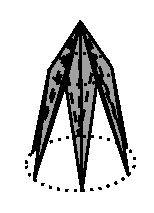
\includegraphics{asy/tent}
\end{wrapfigure}

For a general polyhedral surface, a deformation decreasing the lengths of all edges may not decrease the area.
Moreover, the surface that minimizes the area among all surfaces with a fixed  triangulation might not be saddle;
the symmetric tent shown on the diagram provides an example [see \ncite{petrunin-monthly} for more details].

%%%%%%%%%%%%%%%%%%%%%%%%%%%%%%%%%%%%%%%%%%%%%%%%%%

\parbf{Coherent triangulation.} 
An example is shown on the diagram.
The triangulation of the triangle $[x'y'z']$ has a homothetic triangle $[xyz]$ and the edges
$[xx']$, $[yy']$, $[zz']$, 
$[yx']$, $[zy']$, $[xz']$.

}

\medskip

Assume this triangulation is coherent;
let $f$ be the corresponding piecewise linear convex function.
Without loss of generality we can assume that $f$ vanishes on the boundary of the big triangle.

\begin{wrapfigure}{r}{33 mm}
\vskip0mm
\centering
\includegraphics{mppics/pic-808}
\end{wrapfigure}

From the convexity of $f$ at the edges $[x'y]$,  $[y'z]$ and $[z'x]$, we get 
\[f(x)>f(y)>f(z)>f(x),\]
a contradiction.
\qeds

The problem is discussed in the book of 
Israel Gelfand, 
Mikhail Kapranov 
and Andrei Zelevinsky  \cite[see 7C in][]{GKZ}.
The given example is closely related to the so-called \index{Sch\"onhardt polyhedron}\emph{Sch\"onhardt polyhedron}, an example of a non-convex polyhedron which does not admit a triangulation \cite{schoenhardt}.

%%%%%%%%%%%%%%%%%%%%%%%%%%%%%%%%%%%%%%%%%%%%%%%%%%
\parbf{Sphere with one edge.} 
An example, say $P$, can be found among polyhedral spaces that admit an isometric $\mathbb{S}^1$-action with geodesic orbits.
(Equivalently the cone over $P$ admits a complex structure; 
that is, one can cut simplexes from $\CC^2$ and glue the cone from them so that the complex structures agree on the gluing.)

\medskip

Let us identify $\mathbb{S}^3$ with the unit sphere in the hyperplane $\Pi$ described by $x+y+z=0$ of $\CC^3$.
The symmetric group $S_3$ acts on $\mathbb{S}^3$ by permuting the coordinates.
Take $P=\mathbb{S}^3/S_3$. 

Note that $P$ is a spherical polyhedral space.
Moreover, $P$ is the  underlying space of an orbifold whose isotopy groups are either trivial or $\ZZ_2$.
In particular $P$ is a 3-manifold.
Clearly $P$ is compact and simply connected, in particular it is homeomorphic to the 3-sphere.
(The later can be also seen by parametrizing $P$ using the symmetric polynomials $u=xy+yz+zx$ and $v=xyz$.)


Multiplications by unit complex numbers give an $\mathbb{S}^1$-action on $\mathbb{S}^3$ which commutes with the $S_3$-action.
The singular set $P_s$ of $P$ is the image of the orbit $\mathbb{S}^1\cdot p$ where $p$ is a point fixed by an odd permutation of $S_3$.
In particular $P_s$ is a circle.

Note that the subgroup of even permutations $\ZZ_3\vartriangleleft S_3$ acts freely on $\mathbb{S}^3$.
The quotient space $\mathbb{S}^3/\ZZ_3$ is the double covering of $P$ branching in $P_s$.
That is, a double covering of the sphere $P$ branching in the knot $P_s$ is not simply connected.
Therefore $P_s$ is a nontrivial knot.

(In fact $P_s$ is a trefoil and in the $(u,v)$ coordinates it can be written as $u^3=v^2$.)
\qeds


This construction is given by Dmitri Panov \cite{panov-Kaeler}.

Note that the quotient space $P'=P/\mathbb{S}^1$ is isometric to the doubling of a triangle in $\CP^1=\mathbb{S}^3/\mathbb{S}^1$ with the angles $\tfrac\pi2$, $\tfrac\pi2$ and $\tfrac\pi3$.
Starting with other triangles one may produce $P$ with isometric $\mathbb{S}^1$ and arbitrary torus knot as the singular set.
It can also produce arbitrary long singular sets.
In these examples, the cone over $P$ can be holomorphically parametrized by $\CC^2$ in such a way that its singular set becomes an algebraic curve $u^p=v^q$ in some $(u,v)$-coordinates of $\CC^2$.
Here is a related problem.

\begin{pr}
Construct a complex orbifold with the underlying space homeomorphic to $\CP^2$. 
\end{pr}

The solution of the problem gives the polyhedral metric on $\CP^2$ with nonnegative curvature in the sense of Alexandrov.
It is not known whether the canonical metric on $\CP^2$ can be approximated by such polyhedral metrics or not.


\begin{wrapfigure}{r}{23 mm}
\vskip-4mm
\centering
\includegraphics{asy/thurston-cube}
\end{wrapfigure}

I do not know if such knots exist in Euclidean polyhedral spaces, but there are links.
For example, the Borromean rings can appear as the singular set of a Euclidean polyhedral metric on $\mathbb S^3$.
It can be obtained by gluing each face of a cube to itself
along the reflections with respect to the middle lines shown on the picture. 
This construction is due to William Thurston \cite{thurston}



%%%%%%%%%%%%%%%%%%%%%%%%%%%%%%%%%%%%%%%%%%%%%%%%%%
\parbf{Triangulation of a torus.}
Assume the contrary;
let $\tau$ be a triangulation of the torus with the vertex $z_5$ meeting $5$ triangles,
vertex $z_7$ meeting $7$ triangles 
and every other vertex meeting $6$ triangles.

Let us equip the torus with the flat metric such that each triangle is equilateral.
The metric will have two singular cone points $z_5$ and $z_7$.
The total angle around $z_5$ is $\tfrac53\cdot\pi$
and the total angle around $z_7$ is $\tfrac73\cdot\pi$.
Note that

\begin{cl}{$({*})$}
the holonomy group of the obtained polyhedral metric on the torus is generated by the rotation by $\tfrac\pi3$.
\end{cl}

Indeed, since parallel translation along any loop preserves the directions of the sides of any triangle;
it can only permute it cyclically, which corresponds to rotations by multiple of $\tfrac\pi3$. 
On the other hand, the holonomy of the loop that surrounds $z_5$ is a rotation by $\tfrac\pi3$.

Consider a closed geodesic $\gamma_1$ minimizing the length among all not null-homotopic circles.
Let $\gamma_2$ be another closed geodesic that minimizes the length and is not homotopic to any power of $\gamma_1$.

Note that $\gamma_1$ and $\gamma_2$ intersect at a single point.
Otherwise one could shorten one of them keeping the defining property.

Note that $\gamma_i$ does not contain $z_5$.
In fact no geodesic can pass thru any singular point with a total angle smaller than $2\cdot\pi$.


Assume that $\gamma_i$ passes thru $z_7$.
Then by $({*})$, one of the two angles cut by $\gamma_i$ at $z_7$ is $\pi$.
It follows that one can push $\gamma_i$ aside so that it does not longer pass thru $z_7$, but remains to be a closed geodesic with the same length.

\begin{wrapfigure}{r}{33 mm}
\vskip0mm
\centering
\includegraphics{mppics/pic-810}
\end{wrapfigure}

Cut the torus along $\gamma_1$ and $\gamma_2$.
In the obtained quadrilateral, connect $z_5$ to $z_7$ by a minimizing geodesic and cut along it.
This way we obtain an annulus $\Omega$ with a flat metric.

Note that a neighborhood of the first boundary component is a parallelogram --- it has equal opposite sides and its angles add up to $2\cdot \pi$.
In particular $\Omega$ admits an isometric immersion into the plane.

The second boundary component has to be mapped to a diangle with straight sides and angles $\tfrac\pi3$.
Such diangle does not exist in the plane --- a contradiction.
\qeds

The problem was originally discovered and solved by {\fontencoding{T1}\selectfont Stanislav Jendro\v{l}}
and Ernest Jucovi\v{c} \cite{jendrol-jucovich},
their proof is combinatorial.
The solution described above was given by Rostislav Matveyev \cite{matveyev}.
A complex-analytic proof was found by 
Ivan Izmestiev, 
Robert Kusner, 
G\"unter Rote, 
Boris Springborn 
and John Sullivan \cite{izmestiev-rote-springborn-kusner}.

\begin{wrapfigure}{r}{20 mm}
\vskip0mm
\centering
\includegraphics{mppics/pic-812}
\end{wrapfigure}

There are flat metrics on the torus with 
only two singular points of total angles $\tfrac53\cdot\pi$ and $\tfrac73\cdot\pi$.
Such an example can be obtained by identifying the hexagon on the picture  according to the arrows.
However, the holonomy group of the obtained torus is generated by the rotation by $\tfrac\pi6$. 
In particular, the observation $({*})$ is essential in the proof.

The same argument shows that the
holonomy group of a flat torus with exactly two singular points of total angle $2\cdot(1\pm \tfrac1n)\cdot\pi$ has more than $n$ elements.
In the solution we did the case $n=6$.

If one denotes by $v_m$ the number of vertices in a triangulation of the torus with $m$ incoming edges,
then by Euler's formula, we get
\[\sum_m(m-6)\cdot v_m=0.\leqno({*}{*})\]
Note that this equation says nothing about $v_6$.
It turns out that for almost any sequence $v_3,v_4,\dots$ satisfying $({*}{*})$ one can adjust $v_6$ so that it corresponds to a triangulation of the torus --- the sequence 
\[0,0,1,v_6,1,0,0,\dots\] 
discussed in the problem is the only exception. %???REF

The following problem is harder. 
Recall that the curvature of a point $s$ in a polyhedral surface is defined as $2\cdot\pi-\theta$, where $\theta$ denotes the total angle around~$s$.
Note that all regular points in a polyhedral surface have zero curvature.

\begin{pr}
Let $\Sigma$ be a spherical polyhedral space homeomorphic to the 2-sphere
and $\omega_1,\dots,\omega_n$ be the curvatures of its singular points.
Set
\[\delta_i=\min\set{|\tfrac{\omega_i}2-2\cdot k\cdot\pi|}{k\in\ZZ}.\]
Show that there is a closed polygonal line in the unit sphere with sides 
$\delta_1,\dots,\delta_n$.  
\end{pr}

This problem was stated and solved by Gabirele Mondello and Dmitri Panov \cite{mondello-panov}.
The solution requires another holonomy group ---
it assigns an element of the double covering of $\SO(3)$ (which is $\SU(2)\z=\mathbb{S}^3$) to any loop in $\Sigma$ that avoids singularities.


%%%%%%%%%%%%%%%%%%%%%%%%%%%%%%%%%%%%%%%%%%%%%%%%%%
\parbf{No simple geodesics.}
The curvature of a vertex on the surface of a convex polyhedron
is defined as $2\cdot\pi-\theta$, where $\theta$ is the total angle around the vertex.

By the Gauss--Bonnet formula, a simple closed geodesic cuts the surface into two disks each with total curvature $2\cdot\pi$.
Therefore it is sufficient to construct a convex polyhedron with curvatures of the vertices $\omega_1,\dots,\omega_n$ such that
$2\cdot\pi$ cannot be obtained as sum of some of the $\omega_i$.

An example of that type can be found among the tetrahedra.
\qeds

The problem is due to Gregory Galperin \cite{galperin} 
and rediscovered by Dmitry Fuchs and Serge Tabachnikov \cite[see 20.8 in][]{fuchs-tabachnikov}.
The following problem is closely related.

\begin{pr}
Assume that the surface of convex polyhedron $P$ contains arbitrary long closed simple geodesics. 
Show that $P$ is an \emph{isosceles tetrahedron};
that is, the opposite edges of the tetrahedron are equal.
\end{pr}

The latter statement was proved by Vladimir Protasov [see \ncite{protasov} and also \ncite{akopyan-petrunin}, \ncite{itoh-vilcu}].

